% Options for packages loaded elsewhere
\PassOptionsToPackage{unicode}{hyperref}
\PassOptionsToPackage{hyphens}{url}
\PassOptionsToPackage{dvipsnames,svgnames,x11names}{xcolor}
%
\documentclass[
  a4paperpaper,
]{article}

\usepackage{amsmath,amssymb}
\usepackage{iftex}
\ifPDFTeX
  \usepackage[T1]{fontenc}
  \usepackage[utf8]{inputenc}
  \usepackage{textcomp} % provide euro and other symbols
\else % if luatex or xetex
  \ifXeTeX
    \usepackage{mathspec} % this also loads fontspec
  \else
    \usepackage{unicode-math} % this also loads fontspec
  \fi
  \defaultfontfeatures{Scale=MatchLowercase}
  \defaultfontfeatures[\rmfamily]{Ligatures=TeX,Scale=1}
\fi
\usepackage{lmodern}
\ifPDFTeX\else  
    % xetex/luatex font selection
\fi
% Use upquote if available, for straight quotes in verbatim environments
\IfFileExists{upquote.sty}{\usepackage{upquote}}{}
\IfFileExists{microtype.sty}{% use microtype if available
  \usepackage[]{microtype}
  \UseMicrotypeSet[protrusion]{basicmath} % disable protrusion for tt fonts
}{}
\makeatletter
\@ifundefined{KOMAClassName}{% if non-KOMA class
  \IfFileExists{parskip.sty}{%
    \usepackage{parskip}
  }{% else
    \setlength{\parindent}{0pt}
    \setlength{\parskip}{6pt plus 2pt minus 1pt}}
}{% if KOMA class
  \KOMAoptions{parskip=half}}
\makeatother
\usepackage{xcolor}
\usepackage[top=30mm,left=30mm,right=30mm,heightrounded]{geometry}
\setlength{\emergencystretch}{3em} % prevent overfull lines
\setcounter{secnumdepth}{5}
% Make \paragraph and \subparagraph free-standing
\ifx\paragraph\undefined\else
  \let\oldparagraph\paragraph
  \renewcommand{\paragraph}[1]{\oldparagraph{#1}\mbox{}}
\fi
\ifx\subparagraph\undefined\else
  \let\oldsubparagraph\subparagraph
  \renewcommand{\subparagraph}[1]{\oldsubparagraph{#1}\mbox{}}
\fi

\usepackage{color}
\usepackage{fancyvrb}
\newcommand{\VerbBar}{|}
\newcommand{\VERB}{\Verb[commandchars=\\\{\}]}
\DefineVerbatimEnvironment{Highlighting}{Verbatim}{commandchars=\\\{\}}
% Add ',fontsize=\small' for more characters per line
\usepackage{framed}
\definecolor{shadecolor}{RGB}{241,243,245}
\newenvironment{Shaded}{\begin{snugshade}}{\end{snugshade}}
\newcommand{\AlertTok}[1]{\textcolor[rgb]{0.68,0.00,0.00}{#1}}
\newcommand{\AnnotationTok}[1]{\textcolor[rgb]{0.37,0.37,0.37}{#1}}
\newcommand{\AttributeTok}[1]{\textcolor[rgb]{0.40,0.45,0.13}{#1}}
\newcommand{\BaseNTok}[1]{\textcolor[rgb]{0.68,0.00,0.00}{#1}}
\newcommand{\BuiltInTok}[1]{\textcolor[rgb]{0.00,0.23,0.31}{#1}}
\newcommand{\CharTok}[1]{\textcolor[rgb]{0.13,0.47,0.30}{#1}}
\newcommand{\CommentTok}[1]{\textcolor[rgb]{0.37,0.37,0.37}{#1}}
\newcommand{\CommentVarTok}[1]{\textcolor[rgb]{0.37,0.37,0.37}{\textit{#1}}}
\newcommand{\ConstantTok}[1]{\textcolor[rgb]{0.56,0.35,0.01}{#1}}
\newcommand{\ControlFlowTok}[1]{\textcolor[rgb]{0.00,0.23,0.31}{#1}}
\newcommand{\DataTypeTok}[1]{\textcolor[rgb]{0.68,0.00,0.00}{#1}}
\newcommand{\DecValTok}[1]{\textcolor[rgb]{0.68,0.00,0.00}{#1}}
\newcommand{\DocumentationTok}[1]{\textcolor[rgb]{0.37,0.37,0.37}{\textit{#1}}}
\newcommand{\ErrorTok}[1]{\textcolor[rgb]{0.68,0.00,0.00}{#1}}
\newcommand{\ExtensionTok}[1]{\textcolor[rgb]{0.00,0.23,0.31}{#1}}
\newcommand{\FloatTok}[1]{\textcolor[rgb]{0.68,0.00,0.00}{#1}}
\newcommand{\FunctionTok}[1]{\textcolor[rgb]{0.28,0.35,0.67}{#1}}
\newcommand{\ImportTok}[1]{\textcolor[rgb]{0.00,0.46,0.62}{#1}}
\newcommand{\InformationTok}[1]{\textcolor[rgb]{0.37,0.37,0.37}{#1}}
\newcommand{\KeywordTok}[1]{\textcolor[rgb]{0.00,0.23,0.31}{#1}}
\newcommand{\NormalTok}[1]{\textcolor[rgb]{0.00,0.23,0.31}{#1}}
\newcommand{\OperatorTok}[1]{\textcolor[rgb]{0.37,0.37,0.37}{#1}}
\newcommand{\OtherTok}[1]{\textcolor[rgb]{0.00,0.23,0.31}{#1}}
\newcommand{\PreprocessorTok}[1]{\textcolor[rgb]{0.68,0.00,0.00}{#1}}
\newcommand{\RegionMarkerTok}[1]{\textcolor[rgb]{0.00,0.23,0.31}{#1}}
\newcommand{\SpecialCharTok}[1]{\textcolor[rgb]{0.37,0.37,0.37}{#1}}
\newcommand{\SpecialStringTok}[1]{\textcolor[rgb]{0.13,0.47,0.30}{#1}}
\newcommand{\StringTok}[1]{\textcolor[rgb]{0.13,0.47,0.30}{#1}}
\newcommand{\VariableTok}[1]{\textcolor[rgb]{0.07,0.07,0.07}{#1}}
\newcommand{\VerbatimStringTok}[1]{\textcolor[rgb]{0.13,0.47,0.30}{#1}}
\newcommand{\WarningTok}[1]{\textcolor[rgb]{0.37,0.37,0.37}{\textit{#1}}}

\providecommand{\tightlist}{%
  \setlength{\itemsep}{0pt}\setlength{\parskip}{0pt}}\usepackage{longtable,booktabs,array}
\usepackage{calc} % for calculating minipage widths
% Correct order of tables after \paragraph or \subparagraph
\usepackage{etoolbox}
\makeatletter
\patchcmd\longtable{\par}{\if@noskipsec\mbox{}\fi\par}{}{}
\makeatother
% Allow footnotes in longtable head/foot
\IfFileExists{footnotehyper.sty}{\usepackage{footnotehyper}}{\usepackage{footnote}}
\makesavenoteenv{longtable}
\usepackage{graphicx}
\makeatletter
\def\maxwidth{\ifdim\Gin@nat@width>\linewidth\linewidth\else\Gin@nat@width\fi}
\def\maxheight{\ifdim\Gin@nat@height>\textheight\textheight\else\Gin@nat@height\fi}
\makeatother
% Scale images if necessary, so that they will not overflow the page
% margins by default, and it is still possible to overwrite the defaults
% using explicit options in \includegraphics[width, height, ...]{}
\setkeys{Gin}{width=\maxwidth,height=\maxheight,keepaspectratio}
% Set default figure placement to htbp
\makeatletter
\def\fps@figure{htbp}
\makeatother

\usepackage{fvextra}
\DefineVerbatimEnvironment{Highlighting}{Verbatim}{breaklines,commandchars=\\\{\}}
\DefineVerbatimEnvironment{OutputCode}{Verbatim}{breaklines,commandchars=\\\{\}}
\makeatletter
\@ifpackageloaded{caption}{}{\usepackage{caption}}
\AtBeginDocument{%
\ifdefined\contentsname
  \renewcommand*\contentsname{Índice}
\else
  \newcommand\contentsname{Índice}
\fi
\ifdefined\listfigurename
  \renewcommand*\listfigurename{Lista de Figuras}
\else
  \newcommand\listfigurename{Lista de Figuras}
\fi
\ifdefined\listtablename
  \renewcommand*\listtablename{Lista de Tabelas}
\else
  \newcommand\listtablename{Lista de Tabelas}
\fi
\ifdefined\figurename
  \renewcommand*\figurename{Figura}
\else
  \newcommand\figurename{Figura}
\fi
\ifdefined\tablename
  \renewcommand*\tablename{Tabela}
\else
  \newcommand\tablename{Tabela}
\fi
}
\@ifpackageloaded{float}{}{\usepackage{float}}
\floatstyle{ruled}
\@ifundefined{c@chapter}{\newfloat{codelisting}{h}{lop}}{\newfloat{codelisting}{h}{lop}[chapter]}
\floatname{codelisting}{Listagem}
\newcommand*\listoflistings{\listof{codelisting}{Lista de Listagens}}
\makeatother
\makeatletter
\makeatother
\makeatletter
\@ifpackageloaded{caption}{}{\usepackage{caption}}
\@ifpackageloaded{subcaption}{}{\usepackage{subcaption}}
\makeatother
\ifLuaTeX
\usepackage[bidi=basic]{babel}
\else
\usepackage[bidi=default]{babel}
\fi
\babelprovide[main,import]{portuguese}
% get rid of language-specific shorthands (see #6817):
\let\LanguageShortHands\languageshorthands
\def\languageshorthands#1{}
\ifLuaTeX
  \usepackage{selnolig}  % disable illegal ligatures
\fi
\usepackage{bookmark}

\IfFileExists{xurl.sty}{\usepackage{xurl}}{} % add URL line breaks if available
\urlstyle{same} % disable monospaced font for URLs
\hypersetup{
  pdftitle={Lista 3: Otimização em RNA},
  pdfauthor={César A. Galvão - 190011572},
  pdflang={pt},
  colorlinks=true,
  linkcolor={blue},
  filecolor={Maroon},
  citecolor={Blue},
  urlcolor={Blue},
  pdfcreator={LaTeX via pandoc}}

\title{Lista 3: Otimização em RNA}
\author{César A. Galvão - 190011572}
\date{}

\begin{document}
\maketitle

\section{Questão 1}\label{questuxe3o-1}

Considere a função

\[
f(x_1, x_2) = x_1^4 + x_2^4 + x_1^2x_2+ x_1x_2^2 - 20x_1^2 - 15x_2^2
\]

\noindent para responder os itens a seguir.

~

\subsection{Item a)}\label{item-a}

Apresente um gráfico com as curvas de nível de \(f(x_1, x_2)\). Quantos
pontos críticos a função parece ter? Dica para usuários do R: use a
função \texttt{geom\_contour\_filled()}.

\begin{center}\rule{0.5\linewidth}{0.5pt}\end{center}

~

A Figura~\ref{fig-q1a} apresenta o gráfico com curvas de nível. A
superfície tem 3 pontos de mínimo local e um ponto de mínimo global, que
parece ocorrer próximo de \((-3,-3)\). Se forem considerados pontos de
sela, mais pontos podem ser considerados, como aqueles entre os mínimos
e possívelmente algum ponto próximo da origem, totalizando entre 8 e 9
pontos críticos.

~

\begin{Shaded}
\begin{Highlighting}[]
\CommentTok{\# funcao}
\NormalTok{f }\OtherTok{\textless{}{-}} \ControlFlowTok{function}\NormalTok{(x1, x2) \{}
\NormalTok{  x1}\SpecialCharTok{\^{}}\DecValTok{4} \SpecialCharTok{+}\NormalTok{ x2}\SpecialCharTok{\^{}}\DecValTok{4} \SpecialCharTok{+}\NormalTok{ x1}\SpecialCharTok{\^{}}\DecValTok{2}\SpecialCharTok{*}\NormalTok{x2 }\SpecialCharTok{+}\NormalTok{ x1}\SpecialCharTok{*}\NormalTok{x2}\SpecialCharTok{\^{}}\DecValTok{2} \SpecialCharTok{{-}} \DecValTok{20}\SpecialCharTok{*}\NormalTok{x1}\SpecialCharTok{\^{}}\DecValTok{2} \SpecialCharTok{{-}} \DecValTok{15}\SpecialCharTok{*}\NormalTok{x2}\SpecialCharTok{\^{}}\DecValTok{2}
\NormalTok{\}}
\CommentTok{\# grid dos dados}
\NormalTok{df }\OtherTok{\textless{}{-}} \FunctionTok{tibble}\NormalTok{(}
  \FunctionTok{expand.grid}\NormalTok{(}\AttributeTok{x1 =} \FunctionTok{seq}\NormalTok{(}\SpecialCharTok{{-}}\DecValTok{5}\NormalTok{, }\DecValTok{5}\NormalTok{, }\AttributeTok{length.out =} \DecValTok{100}\NormalTok{),}
              \AttributeTok{x2 =} \FunctionTok{seq}\NormalTok{(}\SpecialCharTok{{-}}\DecValTok{5}\NormalTok{, }\DecValTok{5}\NormalTok{, }\AttributeTok{length.out =} \DecValTok{100}\NormalTok{)),}
  \AttributeTok{f =} \FunctionTok{f}\NormalTok{(x1, x2))}

\NormalTok{surface }\OtherTok{\textless{}{-}} \FunctionTok{ggplot}\NormalTok{() }\SpecialCharTok{+}
  \FunctionTok{geom\_contour\_filled}\NormalTok{(}\AttributeTok{data =}\NormalTok{ df, }\FunctionTok{aes}\NormalTok{(}\AttributeTok{x =}\NormalTok{ x1, }\AttributeTok{y =}\NormalTok{ x2, }\AttributeTok{z =}\NormalTok{ f)) }\SpecialCharTok{+}
  \FunctionTok{labs}\NormalTok{(}\AttributeTok{x =} \FunctionTok{TeX}\NormalTok{(}\StringTok{"$x\_1$"}\NormalTok{), }\AttributeTok{y =} \FunctionTok{TeX}\NormalTok{(}\StringTok{"$x\_2$"}\NormalTok{))}\SpecialCharTok{+}
  \FunctionTok{theme\_minimal}\NormalTok{()}\SpecialCharTok{+}
  \FunctionTok{theme}\NormalTok{(}\AttributeTok{legend.position =} \StringTok{"none"}\NormalTok{,}
        \AttributeTok{panel.grid =} \FunctionTok{element\_blank}\NormalTok{(),}
        \AttributeTok{axis.title.y =} \FunctionTok{element\_text}\NormalTok{(}\AttributeTok{angle =} \DecValTok{0}\NormalTok{, }\AttributeTok{vjust =} \FloatTok{0.5}\NormalTok{))}
\end{Highlighting}
\end{Shaded}

\begin{figure}[H]

\centering{

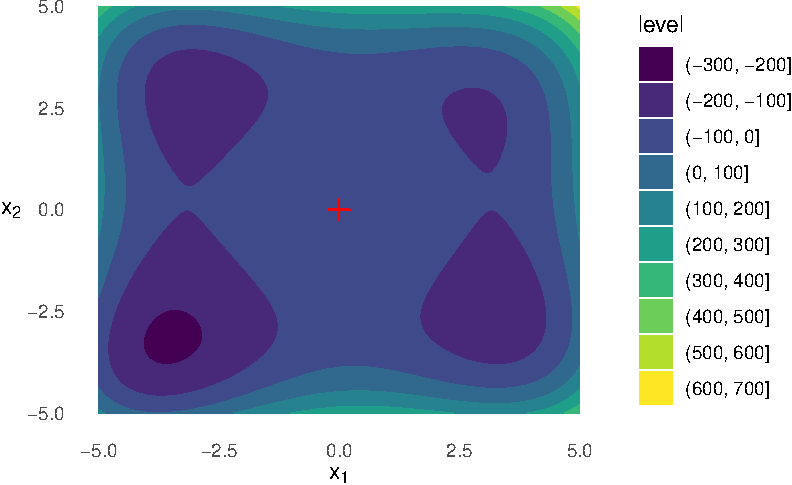
\includegraphics{lista3-resolucao_files/figure-pdf/fig-q1a-1.pdf}

}

\caption{\label{fig-q1a}Curvas de nível de \(f(x_1, x_2)\)}

\end{figure}%

~

\subsection{Item b)}\label{item-b}

Encontre (algericamente) o gradiente de \(f\) em relação ao vetor
\(x = (x_1 , x_2 )\). Isso é,

\[
\nabla_x f(\boldsymbol{x}) = \left( \frac{\partial f}{\partial x_1}, \frac{\partial f}{\partial x_2} \right).
\]

\begin{center}\rule{0.5\linewidth}{0.5pt}\end{center}

~

\begin{align}
 \nabla_x f(\boldsymbol{x}) &= 
    \begin{bmatrix} 
      \frac{\partial f}{\partial x_1} \\ \\
      \frac{\partial f}{\partial x_2} 
    \end{bmatrix} \nonumber \\
  &= \begin{bmatrix} 
        4x_1^3 + 2x_2x_1 + x_2^2 - 40x_1 \\ \\ 
        4x_2^3 + 2x_1x_2 + x_1^2 - 30x_2 
      \end{bmatrix}
\end{align}

~

\subsection{Item c)}\label{item-c}

Crie uma função computacional que implemente o método do gradiente para
minimizar a função emestudo. Permita ao usuário definir a taxa de
aprendizado, o número de passos e o ponto de partida.

\begin{center}\rule{0.5\linewidth}{0.5pt}\end{center}

~

A função \texttt{gradiente()} implementa o método do gradiente para
minimizar a função \(f(x_1, x_2)\). Os argumentos padrão são:

\begin{itemize}
\tightlist
\item
  \(x_0\): o ponto de partida, tomando a origem como padrão;
\item
  \texttt{l.rate}: a taxa de aprendizado, com valor padrão de 0.01;
\item
  \texttt{steps}: o número de passos, com valor padrão de 1000;
\item
  \texttt{keep}: indica se os pontos intermediários devem ser mantidos.
\end{itemize}

A função retorna o ponto de mínimo encontrado depois de \texttt{steps}
passos e única função que a função minimiza é a que foi indicada na
lista.

~

\begin{Shaded}
\begin{Highlighting}[]
\CommentTok{\# funcao do gradiente}
\NormalTok{grad }\OtherTok{\textless{}{-}} \ControlFlowTok{function}\NormalTok{(x) \{}
    \FunctionTok{c}\NormalTok{(}\DecValTok{4}\SpecialCharTok{*}\NormalTok{x[}\DecValTok{1}\NormalTok{]}\SpecialCharTok{\^{}}\DecValTok{3} \SpecialCharTok{+} \DecValTok{2}\SpecialCharTok{*}\NormalTok{x[}\DecValTok{2}\NormalTok{]}\SpecialCharTok{*}\NormalTok{x[}\DecValTok{1}\NormalTok{] }\SpecialCharTok{+}\NormalTok{ x[}\DecValTok{2}\NormalTok{]}\SpecialCharTok{\^{}}\DecValTok{2} \SpecialCharTok{{-}} \DecValTok{40}\SpecialCharTok{*}\NormalTok{x[}\DecValTok{1}\NormalTok{],}
      \DecValTok{4}\SpecialCharTok{*}\NormalTok{x[}\DecValTok{2}\NormalTok{]}\SpecialCharTok{\^{}}\DecValTok{3} \SpecialCharTok{+} \DecValTok{2}\SpecialCharTok{*}\NormalTok{x[}\DecValTok{1}\NormalTok{]}\SpecialCharTok{*}\NormalTok{x[}\DecValTok{2}\NormalTok{] }\SpecialCharTok{+}\NormalTok{ x[}\DecValTok{1}\NormalTok{]}\SpecialCharTok{\^{}}\DecValTok{2} \SpecialCharTok{{-}} \DecValTok{30}\SpecialCharTok{*}\NormalTok{x[}\DecValTok{2}\NormalTok{])}
\NormalTok{  \}}

\NormalTok{gradiente }\OtherTok{\textless{}{-}} \ControlFlowTok{function}\NormalTok{(}\AttributeTok{x0 =} \FunctionTok{c}\NormalTok{(}\DecValTok{0}\NormalTok{,}\DecValTok{0}\NormalTok{), }\AttributeTok{l.rate =} \FloatTok{0.01}\NormalTok{, }\AttributeTok{steps =} \DecValTok{100}\NormalTok{, }\AttributeTok{keep =} \ConstantTok{FALSE}\NormalTok{) \{}
  
  \ControlFlowTok{if}\NormalTok{(keep }\SpecialCharTok{==} \ConstantTok{FALSE}\NormalTok{)\{}
\NormalTok{    x }\OtherTok{\textless{}{-}}\NormalTok{ x0}
    \CommentTok{\# loop padrão}
    \ControlFlowTok{for}\NormalTok{ (i }\ControlFlowTok{in} \DecValTok{1}\SpecialCharTok{:}\NormalTok{steps) \{}
\NormalTok{      x }\OtherTok{\textless{}{-}}\NormalTok{ x }\SpecialCharTok{{-}}\NormalTok{ l.rate }\SpecialCharTok{*} \FunctionTok{grad}\NormalTok{(x)}
\NormalTok{    \}}
\NormalTok{  \} }\ControlFlowTok{else}\NormalTok{ \{}
      \CommentTok{\# loop mantendo pontos intermediários}
\NormalTok{      x }\OtherTok{\textless{}{-}} \FunctionTok{matrix}\NormalTok{(}\ConstantTok{NA}\NormalTok{, }\AttributeTok{nrow =}\NormalTok{ steps}\SpecialCharTok{+}\DecValTok{1}\NormalTok{, }\AttributeTok{ncol =} \DecValTok{2}\NormalTok{)}
\NormalTok{      x[}\DecValTok{1}\NormalTok{,] }\OtherTok{\textless{}{-}}\NormalTok{ x0}
      \ControlFlowTok{for}\NormalTok{ (i }\ControlFlowTok{in} \DecValTok{1}\SpecialCharTok{:}\NormalTok{steps) \{}
\NormalTok{        x[i}\SpecialCharTok{+}\DecValTok{1}\NormalTok{,] }\OtherTok{\textless{}{-}}\NormalTok{ x[i,] }\SpecialCharTok{{-}}\NormalTok{ l.rate }\SpecialCharTok{*} \FunctionTok{grad}\NormalTok{(x[i,])}
\NormalTok{      \}}
\NormalTok{  \}}
  
  \FunctionTok{return}\NormalTok{(x)}
\NormalTok{\}}
\end{Highlighting}
\end{Shaded}

~

\subsection{Item d)}\label{item-d}

Use a função criada no item c) para encontrar o valor obtido pelo método
do gradiente partindo-se do ponto inicial
\(\left(x_1^{(0)} , x_2^{(0)} \right) = (0, 5)\). Use taxa de
aprendizado igual a 0.01 e execute 100 passos.

\begin{center}\rule{0.5\linewidth}{0.5pt}\end{center}

\begin{Shaded}
\begin{Highlighting}[]
\FunctionTok{gradiente}\NormalTok{(}\AttributeTok{x0 =} \FunctionTok{c}\NormalTok{(}\DecValTok{0}\NormalTok{,}\DecValTok{5}\NormalTok{), }\AttributeTok{l.rate =} \FloatTok{0.01}\NormalTok{, }\AttributeTok{steps =} \DecValTok{100}\NormalTok{)}
\end{Highlighting}
\end{Shaded}

\begin{verbatim}
[1] -3.040141  2.865981
\end{verbatim}

\begin{figure}[H]

\centering{

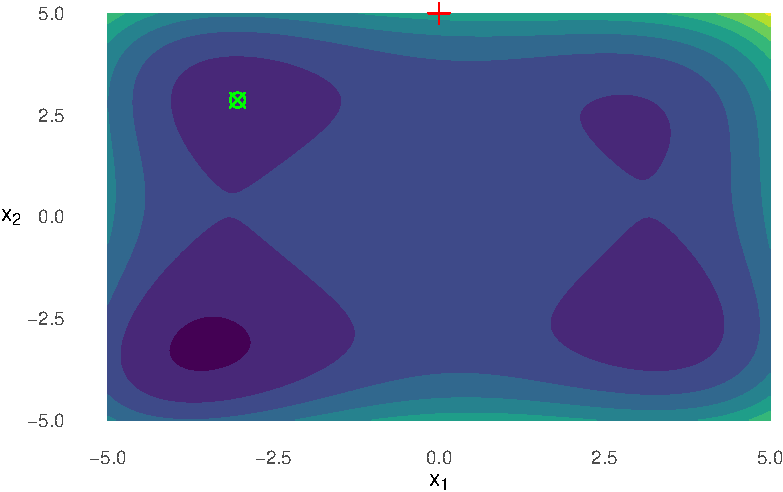
\includegraphics{lista3-resolucao_files/figure-pdf/fig-q1d-1.pdf}

}

\caption{\label{fig-q1d}Ponto final do método do gradiente partindo de
(0,5)}

\end{figure}%

~

\subsection{Item e)}\label{item-e}

Repita o item d), agora com as seguintes taxas de aprendizado: 1, 0.1,
0.01, 0.001, 0.0001. Qual dessas opções lhe parece mais apropriada nesse
caso? Justifique sua resposta.

\begin{center}\rule{0.5\linewidth}{0.5pt}\end{center}

~

A Tabela~\ref{tbl-q1e} apresenta os resultados obtidos para diferentes
taxas de aprendizado. A taxa de aprendizado de 0.01 parece ser a mais
apropriada, pois é a única que converge para o mínimo local da função. A
partir da iteração 22 não é mais possível observar mudanças na direção
do gradiente considerando 6 casas decimentis. As taxas de aprendizado
0.001 e 0.0001 possivelmente convergiriam, mas exigiriam muito mais
passos.

As taxas de aprendizado 1 e 0.1 divergem rapidamente. Suas primeiras
iterações já direcionam o próximo ponto para fora do mapa considerado,
rapidamente indo para infinito. Isso provavelmente ocorre devido à
magnitude do vetor gradiente nos primeiros pontos do algoritmo do
gradiente.

~

\begin{Shaded}
\begin{Highlighting}[]
\NormalTok{q1e\_table }\OtherTok{\textless{}{-}} \FunctionTok{bind\_rows}\NormalTok{(}
  \FunctionTok{as\_tibble}\NormalTok{(}\FunctionTok{gradiente}\NormalTok{(}\AttributeTok{x0 =} \FunctionTok{c}\NormalTok{(}\DecValTok{0}\NormalTok{,}\DecValTok{5}\NormalTok{), }\AttributeTok{l.rate =} \DecValTok{1}\NormalTok{, }\AttributeTok{steps =} \DecValTok{100}\NormalTok{, }\AttributeTok{keep =} \ConstantTok{TRUE}\NormalTok{)),}
  \FunctionTok{as\_tibble}\NormalTok{(}\FunctionTok{gradiente}\NormalTok{(}\AttributeTok{x0 =} \FunctionTok{c}\NormalTok{(}\DecValTok{0}\NormalTok{,}\DecValTok{5}\NormalTok{), }\AttributeTok{l.rate =} \FloatTok{0.1}\NormalTok{, }\AttributeTok{steps =} \DecValTok{100}\NormalTok{, }\AttributeTok{keep =} \ConstantTok{TRUE}\NormalTok{)),}
  \FunctionTok{as\_tibble}\NormalTok{(}\FunctionTok{gradiente}\NormalTok{(}\AttributeTok{x0 =} \FunctionTok{c}\NormalTok{(}\DecValTok{0}\NormalTok{,}\DecValTok{5}\NormalTok{), }\AttributeTok{l.rate =} \FloatTok{0.01}\NormalTok{, }\AttributeTok{steps =} \DecValTok{100}\NormalTok{, }\AttributeTok{keep =} \ConstantTok{TRUE}\NormalTok{)),}
  \FunctionTok{as\_tibble}\NormalTok{(}\FunctionTok{gradiente}\NormalTok{(}\AttributeTok{x0 =} \FunctionTok{c}\NormalTok{(}\DecValTok{0}\NormalTok{,}\DecValTok{5}\NormalTok{), }\AttributeTok{l.rate =} \FloatTok{0.001}\NormalTok{, }\AttributeTok{steps =} \DecValTok{100}\NormalTok{, }\AttributeTok{keep =} \ConstantTok{TRUE}\NormalTok{)),}
  \FunctionTok{as\_tibble}\NormalTok{(}\FunctionTok{gradiente}\NormalTok{(}\AttributeTok{x0 =} \FunctionTok{c}\NormalTok{(}\DecValTok{0}\NormalTok{,}\DecValTok{5}\NormalTok{), }\AttributeTok{l.rate =} \FloatTok{0.0001}\NormalTok{, }\AttributeTok{steps =} \DecValTok{100}\NormalTok{, }\AttributeTok{keep =} \ConstantTok{TRUE}\NormalTok{))}
\NormalTok{) }\SpecialCharTok{\%\textgreater{}\%}
  \FunctionTok{mutate}\NormalTok{(}\AttributeTok{l.rate =} \FunctionTok{rep}\NormalTok{(}\FunctionTok{c}\NormalTok{(}\StringTok{\textquotesingle{}1\textquotesingle{}}\NormalTok{, }\StringTok{\textquotesingle{}0.1\textquotesingle{}}\NormalTok{, }\StringTok{\textquotesingle{}0.01\textquotesingle{}}\NormalTok{, }\StringTok{\textquotesingle{}0.001\textquotesingle{}}\NormalTok{, }\StringTok{\textquotesingle{}0.0001\textquotesingle{}}\NormalTok{), }\AttributeTok{each =} \DecValTok{101}\NormalTok{),}
         \AttributeTok{step =} \FunctionTok{rep}\NormalTok{(}\DecValTok{0}\SpecialCharTok{:}\DecValTok{100}\NormalTok{, }\AttributeTok{times =} \DecValTok{5}\NormalTok{),}
         \FunctionTok{across}\NormalTok{(}\FunctionTok{everything}\NormalTok{(), }\SpecialCharTok{\textasciitilde{}} \FunctionTok{if\_else}\NormalTok{(}\FunctionTok{is.nan}\NormalTok{(.), }\ConstantTok{NA}\NormalTok{, .)))}

\FunctionTok{tibble}\NormalTok{(}
  \AttributeTok{l.rate =} \FunctionTok{c}\NormalTok{(}\StringTok{\textquotesingle{}1\textquotesingle{}}\NormalTok{, }\StringTok{\textquotesingle{}0.1\textquotesingle{}}\NormalTok{, }\StringTok{\textquotesingle{}0.01\textquotesingle{}}\NormalTok{, }\StringTok{\textquotesingle{}0.001\textquotesingle{}}\NormalTok{, }\StringTok{\textquotesingle{}0.0001\textquotesingle{}}\NormalTok{),}
  \AttributeTok{conv =} \FunctionTok{c}\NormalTok{(}\StringTok{"não"}\NormalTok{, }\StringTok{"não"}\NormalTok{, }\StringTok{"sim"}\NormalTok{, }\StringTok{"sim*"}\NormalTok{, }\StringTok{"sim*"}\NormalTok{)}
\NormalTok{) }\SpecialCharTok{\%\textgreater{}\%}
\NormalTok{  knitr}\SpecialCharTok{::}\FunctionTok{kable}\NormalTok{(}
    \AttributeTok{align =} \StringTok{"lc"}\NormalTok{,}
    \AttributeTok{col.names =} \FunctionTok{c}\NormalTok{(}\StringTok{"Learning rate"}\NormalTok{, }\StringTok{"Converge?"}\NormalTok{)}
\NormalTok{  )}
\end{Highlighting}
\end{Shaded}

\begin{longtable}[]{@{}lc@{}}

\caption{\label{tbl-q1e}Resultados do método do gradiente para
diferentes taxas de aprendizado}

\tabularnewline

\toprule\noalign{}
Learning rate & Converge? \\
\midrule\noalign{}
\endhead
\bottomrule\noalign{}
\endlastfoot
1 & não \\
0.1 & não \\
0.01 & sim \\
0.001 & sim* \\
0.0001 & sim* \\

\end{longtable}

~

\subsection{Item f)}\label{item-f}

Fixe a semente do gerador de números aleatórios no valor 123 (se estiver
usando o R, basta executar o código \texttt{set.seed(123)}). Repita
novamente o item d), agora partindo de 20 pontos escolidos
aleatoriamente (uniformemente) no quadrado \(−5 < x_1 , x_2 < 5\).
Refaça o gráfico do item a) e adicione uma linha representando o caminho
percorrido por cada uma das 20 otimizações. Qual foi o percentual de
vezes em que o algoritmo encontrou o mínimo global da função
(despresando um eventual desvio de menor importância)?

\begin{center}\rule{0.5\linewidth}{0.5pt}\end{center}

~

A seguir são exibidos os 20 pontos gerados aleatoriamente e seus pontos
finais. A Figura~\ref{fig-q1f} apresenta o caminho percorrido por cada
uma das 20 otimizações. O percentual de vezes em que o algoritmo
encontrou o mínimo global da função foi de 20\%.

~

\begin{Shaded}
\begin{Highlighting}[]
\CommentTok{\#semente aleatoria}
\FunctionTok{set.seed}\NormalTok{(}\DecValTok{123}\NormalTok{)}
\CommentTok{\# 20 pontos iniciais}
\NormalTok{x0 }\OtherTok{\textless{}{-}} \FunctionTok{tibble}\NormalTok{(}\AttributeTok{x1 =} \FunctionTok{runif}\NormalTok{(}\DecValTok{20}\NormalTok{, }\SpecialCharTok{{-}}\DecValTok{5}\NormalTok{, }\DecValTok{5}\NormalTok{),}
             \AttributeTok{x2 =} \FunctionTok{runif}\NormalTok{(}\DecValTok{20}\NormalTok{, }\SpecialCharTok{{-}}\DecValTok{5}\NormalTok{, }\DecValTok{5}\NormalTok{))}
\CommentTok{\# 20 pontos finais}
\NormalTok{end\_points }\OtherTok{\textless{}{-}}\NormalTok{ x0 }\SpecialCharTok{\%$\%}
  \FunctionTok{map2}\NormalTok{(x1, x2, }\SpecialCharTok{\textasciitilde{}}\FunctionTok{gradiente}\NormalTok{(}\FunctionTok{c}\NormalTok{(.x, .y), }\AttributeTok{l.rate =} \FloatTok{0.01}\NormalTok{, }\AttributeTok{steps =} \DecValTok{100}\NormalTok{)) }\SpecialCharTok{\%\textgreater{}\%}
  \FunctionTok{map}\NormalTok{(., }\SpecialCharTok{\textasciitilde{}} \FunctionTok{t}\NormalTok{(}\FunctionTok{as.matrix}\NormalTok{(.))) }\SpecialCharTok{\%\textgreater{}\%}
  \FunctionTok{map2}\NormalTok{(., }\FunctionTok{seq\_along}\NormalTok{(.), }\SpecialCharTok{\textasciitilde{}} \FunctionTok{as\_tibble}\NormalTok{(.x) }\SpecialCharTok{\%\textgreater{}\%} \FunctionTok{mutate}\NormalTok{(}\AttributeTok{id =}\NormalTok{ .y)) }\SpecialCharTok{\%\textgreater{}\%}
  \FunctionTok{bind\_rows}\NormalTok{() }\SpecialCharTok{\%\textgreater{}\%}
  \FunctionTok{mutate}\NormalTok{(}\AttributeTok{id =} \FunctionTok{as.factor}\NormalTok{(id)) }\SpecialCharTok{\%\textgreater{}\%}
\NormalTok{  rlang}\SpecialCharTok{::}\FunctionTok{set\_names}\NormalTok{(}\FunctionTok{c}\NormalTok{(}\StringTok{"x1"}\NormalTok{, }\StringTok{"x2"}\NormalTok{, }\StringTok{"id"}\NormalTok{))}

\CommentTok{\# resultados}
\NormalTok{paths }\OtherTok{\textless{}{-}}\NormalTok{ x0 }\SpecialCharTok{\%$\%}
  \FunctionTok{map2}\NormalTok{(x1, x2, }\SpecialCharTok{\textasciitilde{}}\FunctionTok{gradiente}\NormalTok{(}\FunctionTok{c}\NormalTok{(.x, .y), }\AttributeTok{l.rate =} \FloatTok{0.01}\NormalTok{, }\AttributeTok{steps =} \DecValTok{100}\NormalTok{, }\AttributeTok{keep =} \ConstantTok{TRUE}\NormalTok{)) }\SpecialCharTok{\%\textgreater{}\%}
  \FunctionTok{map2}\NormalTok{(., }\FunctionTok{seq\_along}\NormalTok{(.), }\SpecialCharTok{\textasciitilde{}} \FunctionTok{as\_tibble}\NormalTok{(.x) }\SpecialCharTok{\%\textgreater{}\%} \FunctionTok{mutate}\NormalTok{(}\AttributeTok{id =}\NormalTok{ .y)) }\SpecialCharTok{\%\textgreater{}\%}
  \FunctionTok{bind\_rows}\NormalTok{() }\SpecialCharTok{\%\textgreater{}\%}
  \FunctionTok{mutate}\NormalTok{(}\AttributeTok{id =} \FunctionTok{as.factor}\NormalTok{(id)) }\SpecialCharTok{\%\textgreater{}\%}
\NormalTok{  rlang}\SpecialCharTok{::}\FunctionTok{set\_names}\NormalTok{(}\FunctionTok{c}\NormalTok{(}\StringTok{"x1"}\NormalTok{, }\StringTok{"x2"}\NormalTok{, }\StringTok{"id"}\NormalTok{))}
  
\CommentTok{\# gráfico}
\CommentTok{\# Assuming x0 has columns x1, x2, and y for labels}
\CommentTok{\# Add the labels to x0 if not already present}
\NormalTok{x0 }\OtherTok{\textless{}{-}}\NormalTok{ x0 }\SpecialCharTok{\%\textgreater{}\%} \FunctionTok{mutate}\NormalTok{(}\AttributeTok{y =} \FunctionTok{paste0}\NormalTok{(}\StringTok{"("}\NormalTok{, }\FunctionTok{round}\NormalTok{(x1, }\DecValTok{2}\NormalTok{), }\StringTok{", "}\NormalTok{, }\FunctionTok{round}\NormalTok{(x2, }\DecValTok{2}\NormalTok{), }\StringTok{")"}\NormalTok{))}

\FunctionTok{ggplot}\NormalTok{() }\SpecialCharTok{+}
  \FunctionTok{geom\_contour\_filled}\NormalTok{(}\AttributeTok{data =}\NormalTok{ df, }\FunctionTok{aes}\NormalTok{(}\AttributeTok{x =}\NormalTok{ x1, }\AttributeTok{y =}\NormalTok{ x2, }\AttributeTok{z =}\NormalTok{ f)) }\SpecialCharTok{+}
  \FunctionTok{geom\_path}\NormalTok{(}\AttributeTok{data =}\NormalTok{ paths, }\FunctionTok{aes}\NormalTok{(}\AttributeTok{x =}\NormalTok{ x1, }\AttributeTok{y =}\NormalTok{ x2, }\AttributeTok{group =}\NormalTok{ id), }\AttributeTok{color =} \StringTok{"yellow"}\NormalTok{, }\AttributeTok{linetype =} \StringTok{"dotted"}\NormalTok{) }\SpecialCharTok{+}
  \FunctionTok{geom\_label}\NormalTok{(}\AttributeTok{data =}\NormalTok{ x0, }\FunctionTok{aes}\NormalTok{(}\AttributeTok{x =}\NormalTok{ x1, }\AttributeTok{y =}\NormalTok{ x2, }\AttributeTok{label =} \FunctionTok{c}\NormalTok{(}\DecValTok{1}\SpecialCharTok{:}\DecValTok{20}\NormalTok{)), }\AttributeTok{color =} \StringTok{"red"}\NormalTok{, }\AttributeTok{size =} \DecValTok{2}\NormalTok{) }\SpecialCharTok{+}
  \FunctionTok{geom\_point}\NormalTok{(}\AttributeTok{data =}\NormalTok{ end\_points, }\FunctionTok{aes}\NormalTok{(}\AttributeTok{x =}\NormalTok{ x1, }\AttributeTok{y =}\NormalTok{ x2), }\AttributeTok{color =} \StringTok{"green"}\NormalTok{, }\AttributeTok{size =} \DecValTok{2}\NormalTok{, }\AttributeTok{shape =} \DecValTok{13}\NormalTok{) }\SpecialCharTok{+}
  \FunctionTok{labs}\NormalTok{(}\AttributeTok{x =} \FunctionTok{TeX}\NormalTok{(}\StringTok{"$x\_1$"}\NormalTok{), }\AttributeTok{y =} \FunctionTok{TeX}\NormalTok{(}\StringTok{"$x\_2$"}\NormalTok{)) }\SpecialCharTok{+}
  \FunctionTok{theme\_minimal}\NormalTok{() }\SpecialCharTok{+}
  \FunctionTok{theme}\NormalTok{(}\AttributeTok{legend.position =} \StringTok{"none"}\NormalTok{,}
        \AttributeTok{panel.grid =} \FunctionTok{element\_blank}\NormalTok{(),}
        \AttributeTok{axis.title.y =} \FunctionTok{element\_text}\NormalTok{(}\AttributeTok{angle =} \DecValTok{0}\NormalTok{, }\AttributeTok{vjust =} \FloatTok{0.5}\NormalTok{))}
\end{Highlighting}
\end{Shaded}

\begin{figure}[H]

\centering{

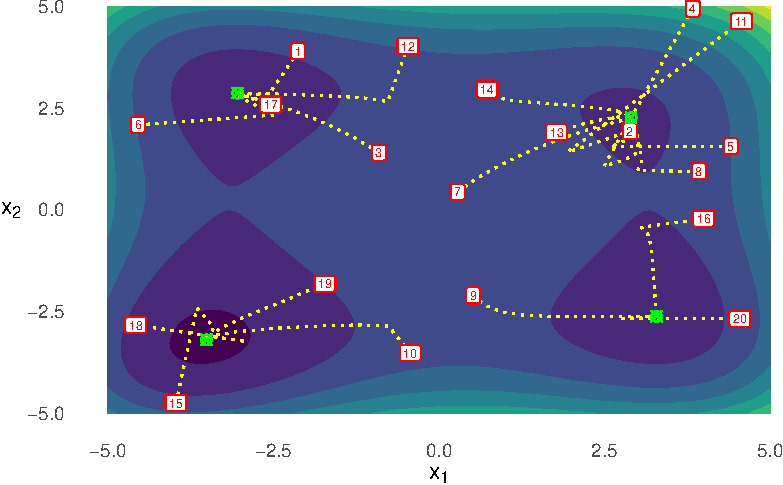
\includegraphics{lista3-resolucao_files/figure-pdf/fig-q1f-1.pdf}

}

\caption{\label{fig-q1f}Caminho percorrido por 20 otimizações}

\end{figure}%

~

\begin{enumerate}
\def\labelenumi{\alph{enumi})}
\setcounter{enumi}{6}
\tightlist
\item
  Repita o item d), substituindo o método do gradiente pelo método do
  gradiente com momento (veja a Seção 8.3.2 do livro \emph{Deep
  Learning}). Use taxa de aprendizado \(\epsilon = 0.01\), parâmetro de
  momento \(\alpha = 0.9\) e velocidade inicial \(v = 0\).
\end{enumerate}

\begin{center}\rule{0.5\linewidth}{0.5pt}\end{center}

~

\begin{Shaded}
\begin{Highlighting}[]
\NormalTok{gradiente\_momento }\OtherTok{\textless{}{-}} \ControlFlowTok{function}\NormalTok{(}\AttributeTok{x0 =} \FunctionTok{c}\NormalTok{(}\DecValTok{0}\NormalTok{,}\DecValTok{0}\NormalTok{), }\AttributeTok{l.rate =} \FloatTok{0.01}\NormalTok{, }\AttributeTok{alpha =} \FloatTok{0.9}\NormalTok{, }\AttributeTok{steps =} \DecValTok{100}\NormalTok{, }\AttributeTok{keep =} \ConstantTok{FALSE}\NormalTok{) \{}
  
  \ControlFlowTok{if}\NormalTok{(keep }\SpecialCharTok{==} \ConstantTok{FALSE}\NormalTok{)\{}
\NormalTok{    x }\OtherTok{\textless{}{-}}\NormalTok{ x0}
\NormalTok{    v }\OtherTok{\textless{}{-}} \DecValTok{0}
    \CommentTok{\# loop padrão}
    \ControlFlowTok{for}\NormalTok{ (i }\ControlFlowTok{in} \DecValTok{1}\SpecialCharTok{:}\NormalTok{steps) \{}
      \CommentTok{\#update velocity}
\NormalTok{      v }\OtherTok{\textless{}{-}}\NormalTok{ alpha }\SpecialCharTok{*}\NormalTok{ v }\SpecialCharTok{{-}}\NormalTok{ l.rate }\SpecialCharTok{*} \FunctionTok{grad}\NormalTok{(x)}
\NormalTok{      x }\OtherTok{\textless{}{-}}\NormalTok{ x }\SpecialCharTok{+}\NormalTok{ v}
\NormalTok{    \}}
\NormalTok{  \} }\ControlFlowTok{else}\NormalTok{ \{}
    \CommentTok{\# loop mantendo pontos intermediários}
\NormalTok{    x }\OtherTok{\textless{}{-}} \FunctionTok{matrix}\NormalTok{(}\ConstantTok{NA}\NormalTok{, }\AttributeTok{nrow =}\NormalTok{ steps}\SpecialCharTok{+}\DecValTok{1}\NormalTok{, }\AttributeTok{ncol =} \DecValTok{2}\NormalTok{)}
\NormalTok{    x[}\DecValTok{1}\NormalTok{,] }\OtherTok{\textless{}{-}}\NormalTok{ x0}
\NormalTok{    v }\OtherTok{\textless{}{-}} \DecValTok{0}
    \ControlFlowTok{for}\NormalTok{ (i }\ControlFlowTok{in} \DecValTok{1}\SpecialCharTok{:}\NormalTok{steps) \{}
      \CommentTok{\#update velocity}
\NormalTok{      v }\OtherTok{\textless{}{-}}\NormalTok{ alpha }\SpecialCharTok{*}\NormalTok{ v }\SpecialCharTok{{-}}\NormalTok{ l.rate }\SpecialCharTok{*} \FunctionTok{grad}\NormalTok{(x[i,])}
\NormalTok{      x[i}\SpecialCharTok{+}\DecValTok{1}\NormalTok{,] }\OtherTok{\textless{}{-}}\NormalTok{ x[i,] }\SpecialCharTok{+}\NormalTok{ v}
\NormalTok{    \}}
\NormalTok{  \}}
  \FunctionTok{return}\NormalTok{(x)}
\NormalTok{\}}

\NormalTok{q1g }\OtherTok{\textless{}{-}} \FunctionTok{gradiente\_momento}\NormalTok{(}\AttributeTok{x0 =} \FunctionTok{c}\NormalTok{(}\DecValTok{0}\NormalTok{,}\DecValTok{5}\NormalTok{))}

\NormalTok{surface}\SpecialCharTok{+}
  \FunctionTok{geom\_point}\NormalTok{(}\FunctionTok{aes}\NormalTok{(}\AttributeTok{x =} \DecValTok{0}\NormalTok{, }\AttributeTok{y =} \DecValTok{5}\NormalTok{), }\AttributeTok{color =} \StringTok{"red"}\NormalTok{, }\AttributeTok{size =} \DecValTok{3}\NormalTok{, }\AttributeTok{shape =} \DecValTok{3}\NormalTok{)}\SpecialCharTok{+}
  \FunctionTok{geom\_point}\NormalTok{(}\FunctionTok{aes}\NormalTok{(}\AttributeTok{x =}\NormalTok{ q1g[}\DecValTok{1}\NormalTok{], }\AttributeTok{y =}\NormalTok{ q1g[}\DecValTok{2}\NormalTok{]), }\AttributeTok{color =} \StringTok{"green"}\NormalTok{, }\AttributeTok{size =} \DecValTok{3}\NormalTok{, }\AttributeTok{shape =} \DecValTok{13}\NormalTok{)}
\end{Highlighting}
\end{Shaded}

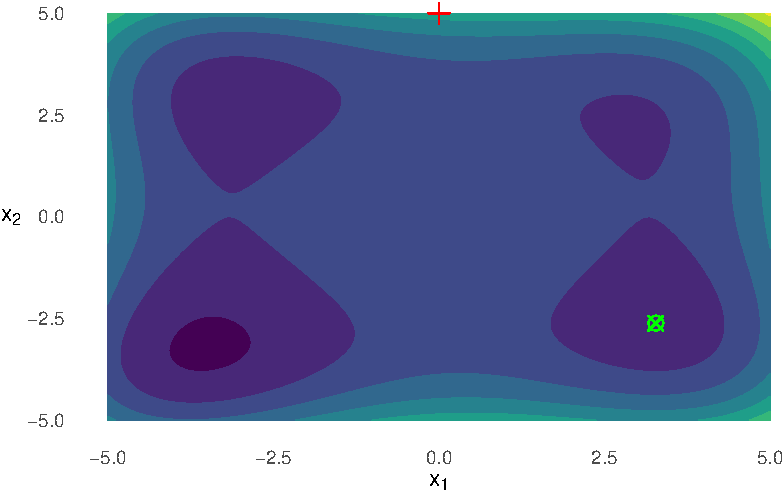
\includegraphics{lista3-resolucao_files/figure-pdf/q1g-1.pdf}

~

\subsection{Item h)}\label{item-h}

Repita o item d), substituindo o método do gradiente pelo método RMSProp
(veja a Seção 8.5.2 do livro Deep Learning). Use taxa de aprendizado
\(\epsilon = 0.001\), taxa de decaimento \(\rho = 0.9\) e constante
\(\delta = 10^{−6}\).

\begin{center}\rule{0.5\linewidth}{0.5pt}\end{center}

~

\begin{Shaded}
\begin{Highlighting}[]
\NormalTok{gradiente\_RMSProp }\OtherTok{\textless{}{-}} \ControlFlowTok{function}\NormalTok{(}\AttributeTok{x0 =} \FunctionTok{c}\NormalTok{(}\DecValTok{0}\NormalTok{,}\DecValTok{0}\NormalTok{), }\AttributeTok{l.rate =} \FloatTok{0.001}\NormalTok{, }\AttributeTok{rho =} \FloatTok{0.9}\NormalTok{, }\AttributeTok{delta =} \DecValTok{10}\SpecialCharTok{\^{}}\NormalTok{(}\SpecialCharTok{{-}}\DecValTok{6}\NormalTok{), }\AttributeTok{steps =} \DecValTok{100}\NormalTok{, }\AttributeTok{keep =} \ConstantTok{FALSE}\NormalTok{) \{}
  
  \ControlFlowTok{if}\NormalTok{(keep }\SpecialCharTok{==} \ConstantTok{FALSE}\NormalTok{)\{}
\NormalTok{    x }\OtherTok{\textless{}{-}}\NormalTok{ x0}
\NormalTok{    s }\OtherTok{\textless{}{-}} \DecValTok{0}
    \CommentTok{\# loop padrão}
    \ControlFlowTok{for}\NormalTok{ (i }\ControlFlowTok{in} \DecValTok{1}\SpecialCharTok{:}\NormalTok{steps) \{}
      \CommentTok{\#update s}
\NormalTok{      s }\OtherTok{\textless{}{-}}\NormalTok{ rho }\SpecialCharTok{*}\NormalTok{ s }\SpecialCharTok{+}\NormalTok{ (}\DecValTok{1} \SpecialCharTok{{-}}\NormalTok{ rho) }\SpecialCharTok{*} \FunctionTok{grad}\NormalTok{(x)}\SpecialCharTok{\^{}}\DecValTok{2}
      \CommentTok{\#parameter update (theta + delta*theta)}
      \CommentTok{\# theta = theta {-} l.rate / sqrt(s + delta) * grad }
\NormalTok{      x }\OtherTok{\textless{}{-}}\NormalTok{ x }\SpecialCharTok{{-}}\NormalTok{ l.rate}\SpecialCharTok{*} \FunctionTok{grad}\NormalTok{(x) }\SpecialCharTok{/} \FunctionTok{sqrt}\NormalTok{(s }\SpecialCharTok{+}\NormalTok{ delta)}
\NormalTok{    \}}
\NormalTok{  \} }\ControlFlowTok{else}\NormalTok{ \{}
    \CommentTok{\# loop mantendo pontos intermediários}
\NormalTok{    x }\OtherTok{\textless{}{-}} \FunctionTok{matrix}\NormalTok{(}\ConstantTok{NA}\NormalTok{, }\AttributeTok{nrow =}\NormalTok{ steps}\SpecialCharTok{+}\DecValTok{1}\NormalTok{, }\AttributeTok{ncol =} \DecValTok{2}\NormalTok{)}
\NormalTok{    x[}\DecValTok{1}\NormalTok{,] }\OtherTok{\textless{}{-}}\NormalTok{ x0}
\NormalTok{    s }\OtherTok{\textless{}{-}} \DecValTok{0}
    \ControlFlowTok{for}\NormalTok{ (i }\ControlFlowTok{in} \DecValTok{1}\SpecialCharTok{:}\NormalTok{steps) \{}
      \CommentTok{\#update s}
\NormalTok{      s }\OtherTok{\textless{}{-}}\NormalTok{ rho }\SpecialCharTok{*}\NormalTok{ s }\SpecialCharTok{+}\NormalTok{ (}\DecValTok{1} \SpecialCharTok{{-}}\NormalTok{ rho) }\SpecialCharTok{*} \FunctionTok{grad}\NormalTok{(x[i,])}\SpecialCharTok{\^{}}\DecValTok{2}
\NormalTok{      x[i}\SpecialCharTok{+}\DecValTok{1}\NormalTok{,] }\OtherTok{\textless{}{-}}\NormalTok{ x[i,] }\SpecialCharTok{{-}}\NormalTok{ l.rate}\SpecialCharTok{*} \FunctionTok{grad}\NormalTok{(x[i,])}\SpecialCharTok{/}\FunctionTok{sqrt}\NormalTok{(s }\SpecialCharTok{+}\NormalTok{ delta) }
\NormalTok{    \}}
\NormalTok{  \}}
  \FunctionTok{return}\NormalTok{(x)}
\NormalTok{\}}

\NormalTok{q1h }\OtherTok{\textless{}{-}} \FunctionTok{gradiente\_RMSProp}\NormalTok{(}\AttributeTok{x0 =} \FunctionTok{c}\NormalTok{(}\DecValTok{0}\NormalTok{,}\DecValTok{5}\NormalTok{), }\AttributeTok{keep =} \ConstantTok{FALSE}\NormalTok{)}

\NormalTok{surface}\SpecialCharTok{+}
  \FunctionTok{geom\_point}\NormalTok{(}\FunctionTok{aes}\NormalTok{(}\AttributeTok{x =} \DecValTok{0}\NormalTok{, }\AttributeTok{y =} \DecValTok{5}\NormalTok{), }\AttributeTok{color =} \StringTok{"red"}\NormalTok{, }\AttributeTok{size =} \DecValTok{3}\NormalTok{, }\AttributeTok{shape =} \DecValTok{3}\NormalTok{)}\SpecialCharTok{+}
  \FunctionTok{geom\_point}\NormalTok{(}\FunctionTok{aes}\NormalTok{(}\AttributeTok{x =}\NormalTok{ q1h[}\DecValTok{1}\NormalTok{], }\AttributeTok{y =}\NormalTok{ q1h[}\DecValTok{2}\NormalTok{]), }\AttributeTok{color =} \StringTok{"green"}\NormalTok{, }\AttributeTok{size =} \DecValTok{3}\NormalTok{, }\AttributeTok{shape =} \DecValTok{13}\NormalTok{)}
\end{Highlighting}
\end{Shaded}

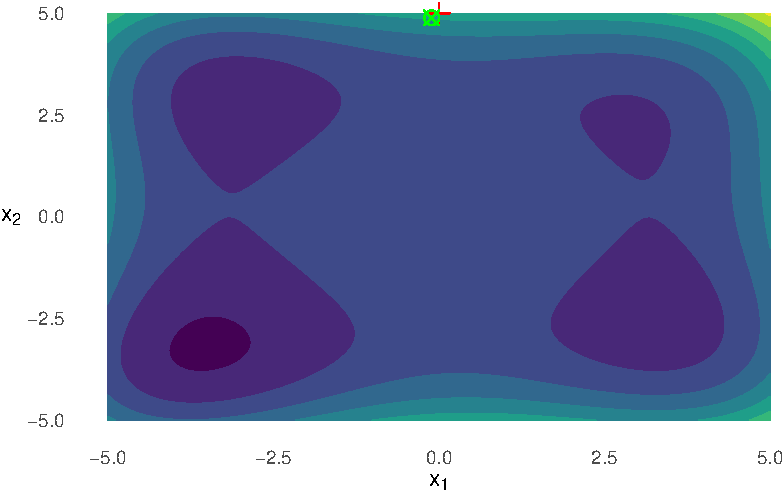
\includegraphics{lista3-resolucao_files/figure-pdf/q1h-1.pdf}

~

\subsection{Item i)}\label{item-i}

Repita o item d), substituindo o método do gradiente pelo método ADAM
(veja a Seção 8.5.3 do livro Deep Learning). Use taxa de aprendizado
\(\epsilon = 0.001\) e taxas de decaimento \(\rho1 = 0.9\) e
\(\rho_2 = 0.999\).

~

\begin{Shaded}
\begin{Highlighting}[]
\NormalTok{gradiente\_ADAM }\OtherTok{\textless{}{-}} \ControlFlowTok{function}\NormalTok{(}\AttributeTok{x0 =} \FunctionTok{c}\NormalTok{(}\DecValTok{0}\NormalTok{,}\DecValTok{0}\NormalTok{), }\AttributeTok{l.rate =} \FloatTok{0.001}\NormalTok{, }\AttributeTok{rho1 =} \FloatTok{0.9}\NormalTok{, }\AttributeTok{rho2 =} \FloatTok{0.999}\NormalTok{, }\AttributeTok{delta =} \DecValTok{10}\SpecialCharTok{\^{}}\NormalTok{(}\SpecialCharTok{{-}}\DecValTok{6}\NormalTok{), }\AttributeTok{steps =} \DecValTok{100}\NormalTok{, }\AttributeTok{keep =} \ConstantTok{FALSE}\NormalTok{) \{}
  
  \ControlFlowTok{if}\NormalTok{(keep }\SpecialCharTok{==} \ConstantTok{FALSE}\NormalTok{)\{}
\NormalTok{    x }\OtherTok{\textless{}{-}}\NormalTok{ x0}
    \CommentTok{\# initialize moment variables}
\NormalTok{    s }\OtherTok{\textless{}{-}} \DecValTok{0}
\NormalTok{    r }\OtherTok{\textless{}{-}} \DecValTok{0}
    \CommentTok{\# loop padrão}
    \ControlFlowTok{for}\NormalTok{ (i }\ControlFlowTok{in} \DecValTok{1}\SpecialCharTok{:}\NormalTok{steps) \{}
      \CommentTok{\#update first moment estimate}
\NormalTok{      s }\OtherTok{\textless{}{-}}\NormalTok{ rho1 }\SpecialCharTok{*}\NormalTok{ s }\SpecialCharTok{+}\NormalTok{ (}\DecValTok{1} \SpecialCharTok{{-}}\NormalTok{ rho1) }\SpecialCharTok{*} \FunctionTok{grad}\NormalTok{(x)}
      \CommentTok{\# update second moment estimate}
\NormalTok{      r }\OtherTok{\textless{}{-}}\NormalTok{ rho2 }\SpecialCharTok{*}\NormalTok{ r }\SpecialCharTok{+}\NormalTok{ (}\DecValTok{1} \SpecialCharTok{{-}}\NormalTok{ rho2) }\SpecialCharTok{*} \FunctionTok{grad}\NormalTok{(x)}\SpecialCharTok{\^{}}\DecValTok{2}
      \CommentTok{\#correct bias in first moment}
\NormalTok{      s\_hat }\OtherTok{\textless{}{-}}\NormalTok{ s }\SpecialCharTok{/}\NormalTok{ (}\DecValTok{1} \SpecialCharTok{{-}}\NormalTok{ rho1}\SpecialCharTok{\^{}}\NormalTok{i)}
      \CommentTok{\#correct bias in second moment}
\NormalTok{      r\_hat }\OtherTok{\textless{}{-}}\NormalTok{ r }\SpecialCharTok{/}\NormalTok{ (}\DecValTok{1} \SpecialCharTok{{-}}\NormalTok{ rho2}\SpecialCharTok{\^{}}\NormalTok{i)}
      \CommentTok{\#apply update (theta = theta + delta*theta)}
      \CommentTok{\# delta*theta = {-}l.rate*(s\_hat) *(sqrt(r\_hat) + delta)}
\NormalTok{      x }\OtherTok{\textless{}{-}}\NormalTok{ x }\SpecialCharTok{{-}}\NormalTok{ l.rate}\SpecialCharTok{*}\NormalTok{s\_hat }\SpecialCharTok{/}\NormalTok{ ((}\FunctionTok{sqrt}\NormalTok{(r\_hat) }\SpecialCharTok{+}\NormalTok{ delta))}
\NormalTok{    \}}
\NormalTok{  \} }\ControlFlowTok{else}\NormalTok{ \{}
    \CommentTok{\# loop mantendo pontos intermediários}
\NormalTok{    x }\OtherTok{\textless{}{-}} \FunctionTok{matrix}\NormalTok{(}\ConstantTok{NA}\NormalTok{, }\AttributeTok{nrow =}\NormalTok{ steps}\SpecialCharTok{+}\DecValTok{1}\NormalTok{, }\AttributeTok{ncol =} \DecValTok{2}\NormalTok{)}
\NormalTok{    x[}\DecValTok{1}\NormalTok{,] }\OtherTok{\textless{}{-}}\NormalTok{ x0}
\NormalTok{    s }\OtherTok{\textless{}{-}} \DecValTok{0}
\NormalTok{    r }\OtherTok{\textless{}{-}} \DecValTok{0}
    \ControlFlowTok{for}\NormalTok{ (i }\ControlFlowTok{in} \DecValTok{1}\SpecialCharTok{:}\NormalTok{steps) \{}
      \CommentTok{\#update m and v}
\NormalTok{      s }\OtherTok{\textless{}{-}}\NormalTok{ rho1 }\SpecialCharTok{*}\NormalTok{ s }\SpecialCharTok{+}\NormalTok{ (}\DecValTok{1} \SpecialCharTok{{-}}\NormalTok{ rho1) }\SpecialCharTok{*} \FunctionTok{grad}\NormalTok{(x[i,])}
\NormalTok{      r }\OtherTok{\textless{}{-}}\NormalTok{ rho2 }\SpecialCharTok{*}\NormalTok{ r }\SpecialCharTok{+}\NormalTok{ (}\DecValTok{1} \SpecialCharTok{{-}}\NormalTok{ rho2) }\SpecialCharTok{*} \FunctionTok{grad}\NormalTok{(x[i,])}\SpecialCharTok{\^{}}\DecValTok{2}
      \CommentTok{\#bias correction}
\NormalTok{      s\_hat }\OtherTok{\textless{}{-}}\NormalTok{ s }\SpecialCharTok{/}\NormalTok{ (}\DecValTok{1} \SpecialCharTok{{-}}\NormalTok{ rho1}\SpecialCharTok{\^{}}\NormalTok{i)}
\NormalTok{      r\_hat }\OtherTok{\textless{}{-}}\NormalTok{ r }\SpecialCharTok{/}\NormalTok{ (}\DecValTok{1} \SpecialCharTok{{-}}\NormalTok{ rho2}\SpecialCharTok{\^{}}\NormalTok{i)}
      \CommentTok{\#parameter update}
\NormalTok{      x[i}\SpecialCharTok{+}\DecValTok{1}\NormalTok{,] }\OtherTok{\textless{}{-}}\NormalTok{ x[i,] }\SpecialCharTok{{-}}\NormalTok{ l.rate}\SpecialCharTok{*}\NormalTok{s\_hat }\SpecialCharTok{/}\NormalTok{ ((}\FunctionTok{sqrt}\NormalTok{(r\_hat) }\SpecialCharTok{+}\NormalTok{ delta))}
\NormalTok{    \}}
\NormalTok{  \}}
  
  \FunctionTok{return}\NormalTok{(x)}
\NormalTok{\}}

\NormalTok{q1j }\OtherTok{\textless{}{-}} \FunctionTok{gradiente\_ADAM}\NormalTok{(}\AttributeTok{x0 =} \FunctionTok{c}\NormalTok{(}\DecValTok{0}\NormalTok{,}\DecValTok{5}\NormalTok{), }\AttributeTok{keep =} \ConstantTok{FALSE}\NormalTok{)}

\NormalTok{surface}\SpecialCharTok{+}
  \FunctionTok{geom\_point}\NormalTok{(}\FunctionTok{aes}\NormalTok{(}\AttributeTok{x =} \DecValTok{0}\NormalTok{, }\AttributeTok{y =} \DecValTok{5}\NormalTok{), }\AttributeTok{color =} \StringTok{"red"}\NormalTok{, }\AttributeTok{size =} \DecValTok{3}\NormalTok{, }\AttributeTok{shape =} \DecValTok{3}\NormalTok{)}\SpecialCharTok{+}
  \FunctionTok{geom\_point}\NormalTok{(}\FunctionTok{aes}\NormalTok{(}\AttributeTok{x =}\NormalTok{ q1j[}\DecValTok{1}\NormalTok{], }\AttributeTok{y =}\NormalTok{ q1j[}\DecValTok{2}\NormalTok{]), }\AttributeTok{color =} \StringTok{"green"}\NormalTok{, }\AttributeTok{size =} \DecValTok{3}\NormalTok{, }\AttributeTok{shape =} \DecValTok{13}\NormalTok{)}
\end{Highlighting}
\end{Shaded}

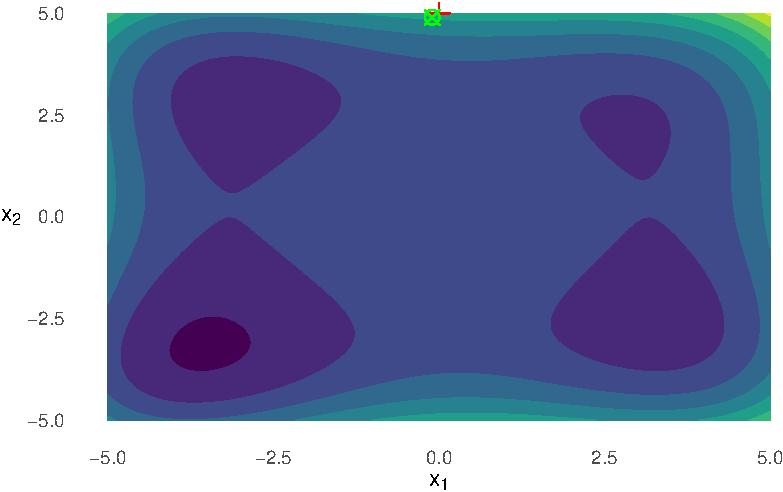
\includegraphics{lista3-resolucao_files/figure-pdf/q1i-1.pdf}

~

\subsection{Item j)}\label{item-j}

Apresente graficamente, em uma única figura, os caminhos percorridos
pelas otimizações executadas nos itens d), g), h) e i).

\begin{Shaded}
\begin{Highlighting}[]
\NormalTok{x0 }\OtherTok{\textless{}{-}} \FunctionTok{c}\NormalTok{(}\DecValTok{0}\NormalTok{,}\DecValTok{5}\NormalTok{)}

\NormalTok{paths }\OtherTok{\textless{}{-}} \FunctionTok{bind\_rows}\NormalTok{(}
  \FunctionTok{as\_tibble}\NormalTok{(}\FunctionTok{gradiente}\NormalTok{(x0, }\AttributeTok{keep =} \ConstantTok{TRUE}\NormalTok{)),}
  \FunctionTok{as\_tibble}\NormalTok{(}\FunctionTok{gradiente\_momento}\NormalTok{(x0, }\AttributeTok{keep =} \ConstantTok{TRUE}\NormalTok{)),}
  \FunctionTok{as\_tibble}\NormalTok{(}\FunctionTok{gradiente\_RMSProp}\NormalTok{(x0, }\AttributeTok{keep =} \ConstantTok{TRUE}\NormalTok{)),}
  \FunctionTok{as\_tibble}\NormalTok{(}\FunctionTok{gradiente\_ADAM}\NormalTok{(x0, }\AttributeTok{keep =} \ConstantTok{TRUE}\NormalTok{))}
\NormalTok{) }\SpecialCharTok{\%\textgreater{}\%}
  \FunctionTok{mutate}\NormalTok{(}
    \AttributeTok{metodo =} \FunctionTok{rep}\NormalTok{(}\FunctionTok{c}\NormalTok{(}\StringTok{"GD"}\NormalTok{, }\StringTok{"Momento"}\NormalTok{, }\StringTok{"RSMProp"}\NormalTok{, }\StringTok{"Adam"}\NormalTok{), }\AttributeTok{each =} \DecValTok{101}\NormalTok{)}
\NormalTok{  ) }\SpecialCharTok{\%\textgreater{}\%}
\NormalTok{  rlang}\SpecialCharTok{::}\FunctionTok{set\_names}\NormalTok{(}\StringTok{"x1"}\NormalTok{, }\StringTok{"x2"}\NormalTok{, }\StringTok{"id"}\NormalTok{)}

\NormalTok{endpoints }\OtherTok{\textless{}{-}}\NormalTok{ paths[}\FunctionTok{c}\NormalTok{(}\DecValTok{101}\NormalTok{, }\DecValTok{202}\NormalTok{, }\DecValTok{303}\NormalTok{, }\DecValTok{404}\NormalTok{),]}

\FunctionTok{ggplot}\NormalTok{() }\SpecialCharTok{+}
  \FunctionTok{geom\_contour\_filled}\NormalTok{(}\AttributeTok{data =}\NormalTok{ df, }\FunctionTok{aes}\NormalTok{(}\AttributeTok{x =}\NormalTok{ x1, }\AttributeTok{y =}\NormalTok{ x2, }\AttributeTok{z =}\NormalTok{ f), }\AttributeTok{show.legend =} \ConstantTok{FALSE}\NormalTok{) }\SpecialCharTok{+}
  \FunctionTok{geom\_path}\NormalTok{(}\AttributeTok{data =}\NormalTok{ paths, }\FunctionTok{aes}\NormalTok{(}\AttributeTok{x =}\NormalTok{ x1, }\AttributeTok{y =}\NormalTok{ x2, }\AttributeTok{group =}\NormalTok{ id, }\AttributeTok{color =}\NormalTok{ id)) }\SpecialCharTok{+}
  \FunctionTok{geom\_point}\NormalTok{(}\AttributeTok{data =}\NormalTok{ endpoints, }\FunctionTok{aes}\NormalTok{(}\AttributeTok{x =}\NormalTok{ x1, }\AttributeTok{y =}\NormalTok{ x2), }\AttributeTok{color =} \StringTok{"green"}\NormalTok{, }\AttributeTok{size =} \DecValTok{2}\NormalTok{, }\AttributeTok{shape =} \DecValTok{13}\NormalTok{) }\SpecialCharTok{+}
  \FunctionTok{labs}\NormalTok{(}\AttributeTok{x =} \FunctionTok{TeX}\NormalTok{(}\StringTok{"$x\_1$"}\NormalTok{), }\AttributeTok{y =} \FunctionTok{TeX}\NormalTok{(}\StringTok{"$x\_2$"}\NormalTok{), }\AttributeTok{color =} \StringTok{"Otimização"}\NormalTok{) }\SpecialCharTok{+}
  \FunctionTok{theme\_minimal}\NormalTok{() }\SpecialCharTok{+}
  \FunctionTok{theme}\NormalTok{(}\AttributeTok{panel.grid =} \FunctionTok{element\_blank}\NormalTok{(),}
        \AttributeTok{axis.title.y =} \FunctionTok{element\_text}\NormalTok{(}\AttributeTok{angle =} \DecValTok{0}\NormalTok{, }\AttributeTok{vjust =} \FloatTok{0.5}\NormalTok{),}
        \AttributeTok{legend.position =} \StringTok{"bottom"}\NormalTok{)}
\end{Highlighting}
\end{Shaded}

\begin{figure}[H]

\centering{

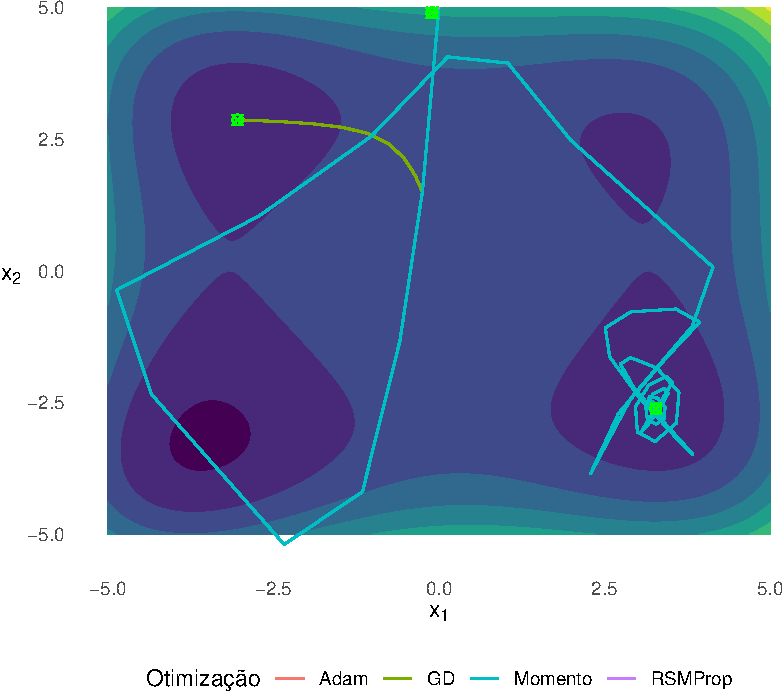
\includegraphics{lista3-resolucao_files/figure-pdf/fig-q1j-1.pdf}

}

\caption{\label{fig-q1j}Caminhos percorridos pelas otimizações
executadas nos itens d), g), h) e i)}

\end{figure}%



\end{document}
